\documentclass[14pt, a4paper]{extarticle}

\usepackage{my_GOST}
\usepackage{hyperref}
\usepackage{listings}
\usepackage{array}
\usepackage{caption}
\hypersetup{
	pdftex,
	colorlinks = true,
	linkcolor = black,
	filecolor = magenta,
	citecolor = green,      
	urlcolor = cyan,
}

% к таблице и листингу подпись сверху, перед каждым иллюстративным материалом анонсировать
% написатьт в квадратных скобках к рекурсии комментарием что это метод и понятно почему вызываем его снова
\definecolor{mylightgray}{RGB}{240,240,240}
\definecolor{mygreen}{rgb}{0,0.6,0}
\definecolor{mygray}{rgb}{0.5,0.5,0.5}
\definecolor{mymauve}{rgb}{0.58,0,0.82}

\lstset{
	backgroundcolor=\color{mylightgray},rulecolor=\color{red},  % choose the background color; you must add \usepackage{color} or \usepackage{xcolor}; should come as last argument
	basicstyle=\footnotesize\ttfamily,        % the size of the fonts that are used for the code
	breakatwhitespace=false,         % sets if automatic breaks should only happen at whitespace
	breaklines=true,                 % sets automatic line breaking
	captionpos=t,                    % sets the caption-position to bottom
	commentstyle=\color{mygreen},    % comment style
	extendedchars=false,              % lets you use non-ASCII characters; for 8-bits encodings only, does not work with UTF-8
	firstnumber=0,                % start line enumeration with line 1000
	frame=shadowbox,
	%rulesepcolor=\color{green},	                   % adds a frame around the code
	keepspaces=true,                 % keeps spaces in text, useful for keeping indentation of code (possibly needs columns=flexible)
	keywordstyle=\color{blue}\textbf,       % keyword style
	language=C++,                 % the language of the code
	morekeywords={*,...},            % if you want to add more keywords to the set
	numbers=left,                    % where to put the line-numbers; possible values are (none, left, right)
	numbersep=5pt,                   % how far the line-numbers are from the code
	numberstyle=\scriptsize\color{mygray}, % the style that is used for the line-numbers
	rulecolor=\color{black},         % if not set, the frame-color may be changed on line-breaks within not-black text (e.g. comments (green here))
	showspaces=false,                % show spaces everywhere adding particular underscores; it overrides 'showstringspaces'
	showstringspaces=false,          % underline spaces within strings only
	showtabs=false,                  % show tabs within strings adding particular underscores
	stepnumber=1,                    % the step between two line-numbers. If it's 1, each line will be numbered
	stringstyle=\color{mymauve},     % string literal style
	tabsize=4,	                   % sets default tabsize to 2 spaces
	title=\lstname                   % show the filename of files included with \lstinputlisting; also try caption instead of title
}
\usepackage{YATPR}

\usepackage{float}

\begin{document}
\begin{titlepage}
	\newgeometry{pdftex, left=2cm, right=2cm, top=2.5cm, bottom=2.5cm}
	\fontsize{12pt}{12pt}\selectfont
	\noindent \begin{minipage}{0.15\textwidth}
		
\includegraphics[width=\linewidth]{pictures/b_logo.jpg}
	\end{minipage}
	\noindent\begin{minipage}{0.9\textwidth}\centering
		\textbf{Министерство науки и высшего образования Российской Федерации}\\
		\textbf{Федеральное государственное бюджетное образовательное учреждение высшего образования}\\
		\textbf{«Московский государственный технический университет имени Н.Э.~Баумана}\\
		\textbf{(национальный исследовательский университет)»}\\
		\textbf{(МГТУ им. Н.Э.~Баумана)}
	\end{minipage}
	
	\noindent\rule{18cm}{3pt}
	\newline\newline
	\noindent ФАКУЛЬТЕТ $\underline{\text{«Информатика и системы управления»}}$ \newline\newline
	\noindent КАФЕДРА $\underline{\text{«Программное обеспечение ЭВМ и информационные технологии»}}$\newline\newline\newline\newline\newline\newline\newline
	
	
	\begin{center}
		\Large\textbf{Отчет по лабораторной работе №5}\newline
	\end{center}
	
	\noindent\textbf{Название} $\underline{\text{~Моделирование работы информационного центра~~~~~~~~~}}$\newline\newline\newline
	\noindent\textbf{Дисциплина} $\underline{\text{~Моделирование~~~~~~~~}}$\newline\newline
	\noindent\textbf{Студент} $\underline{\text{Зайцева А. А.~~~~~~~~~~~~~~~~~~~~~~~~~~~~~~~~~~~~~~~~~}}$\newline\newline
	\noindent\textbf{Группа} $\underline{\text{ИУ7-72Б~~~~~~~~~~~~~~~~~~~~~~~~~~~~~~~~~~~~~~~~~~~~}}$\newline\newline
	\noindent\textbf{Оценка (баллы)} $\underline{\text{~~~~~~~~~~~~~~~~~~~~~~~~~~~~~~~~~~~~~~~~~~~~~~~~~}}$\newline\newline
	\noindent\textbf{Преподаватель}$\underline{\text{~Рудаков И. В.~~~~~~~~~~}}$\newline
	
	\begin{center}
		\vfill
		Москва~---~\the\year
		~г.
	\end{center}
 \restoregeometry
\end{titlepage}


\setcounter{page}{2}

\section{Задание}
Разработать программу для построения графиков функции распределения и функции плотности распределения для следующих распределений: 
\begin{itemize}
	\item равномерное распределение;
	\item распределение Пуассона (вариант 3).
\end{itemize} 

Разработать графический интерфейс, предоставляющий возможность выбора закона распределения и указания его параметров.

\section{Теоретические сведения}

\subsection{Равномерное распределение}

Функция плотности распределения $f(x)$ случайной величины $X$, имеющей равномерное распределение на отрезке $[a, b]$ ($X \sim R(a, b)$), где $a, b \in R$, имеет следующий вид:
\begin{equation}
	f(x)=\begin{cases}
		\frac{1}{b - a}, & x \in [a, b] \\
		0, & \text{иначе}.
	\end{cases}
\end{equation}

Соответствующая функция распределения $F(x) = \int_{-\infty}^{x}f(t)dt$ принимает вид: 
\begin{equation}
	F(x)=\begin{cases}
		0, & x < a, \\
		\frac{x - a}{b - a}, & x \in [a, b] \\
		1, & x > b
	\end{cases}
\end{equation}


\subsection{Распределение Пуассона}

Биномиальное распределение с параметрами $n$ и $p$ -- это распределение количества <<успехов>> в последовательности из $n$ независимых случайных экспериментов, таких, что вероятность <<успеха>> в каждом из них постоянна и равна $p$.

Распределение Пуассона -- это частный случай биномиального распределения при $n \gg 0$ и $p \to 0$. Распределение Пуассона также называют законом <<редких>> событий, так как оно всегда проявляется там, где производится большое число испытаний, в каждом из которых с малой вероятностью происходит <<редкое>> событие.


Дискретная случайная величина $X$ имеет закон распределения Пуассона с параметром $\lambda$ ($X \sim \Pi(\lambda)$), где $\lambda > 0$, если она принимает значения $0, 1, 2,...$ с вероятностями:

\begin{equation}
	P(X = k)= e^{-\lambda}\frac{\lambda^{k}}{k!}, \quad k \in \{0, 1, 2, ...\}
\end{equation}


Параметр $\lambda$ распределения Пуассона -- это среднее количество успешных испытаний в заданной области возможных исходов. 


Соответствующая функция распределения принимает вид:

\begin{equation}
F(x) = P(X < x) = \sum_{k=0}^{x-1}P(X = k) = e^{-\lambda}\sum_{k=0}^{x-1}\frac{\lambda^{k}}{k!} 
\end{equation}

Для дискретной случайной величины не существует функции плотности распределения вероятностей. 

\section{Результаты работы программы}


\subsection{Равномерное распределение}

На рисунках \ref{fig:u1} и \ref{fig:u2} приведены результаты построения графиков функций плотности $f(x)$ и распределения $F(x)$ для случайных величин $X \sim R(-4, 4)$ и $X \sim R(1, 3)$, соответственно.

\begin{figure}[h!]
	\begin{center}
		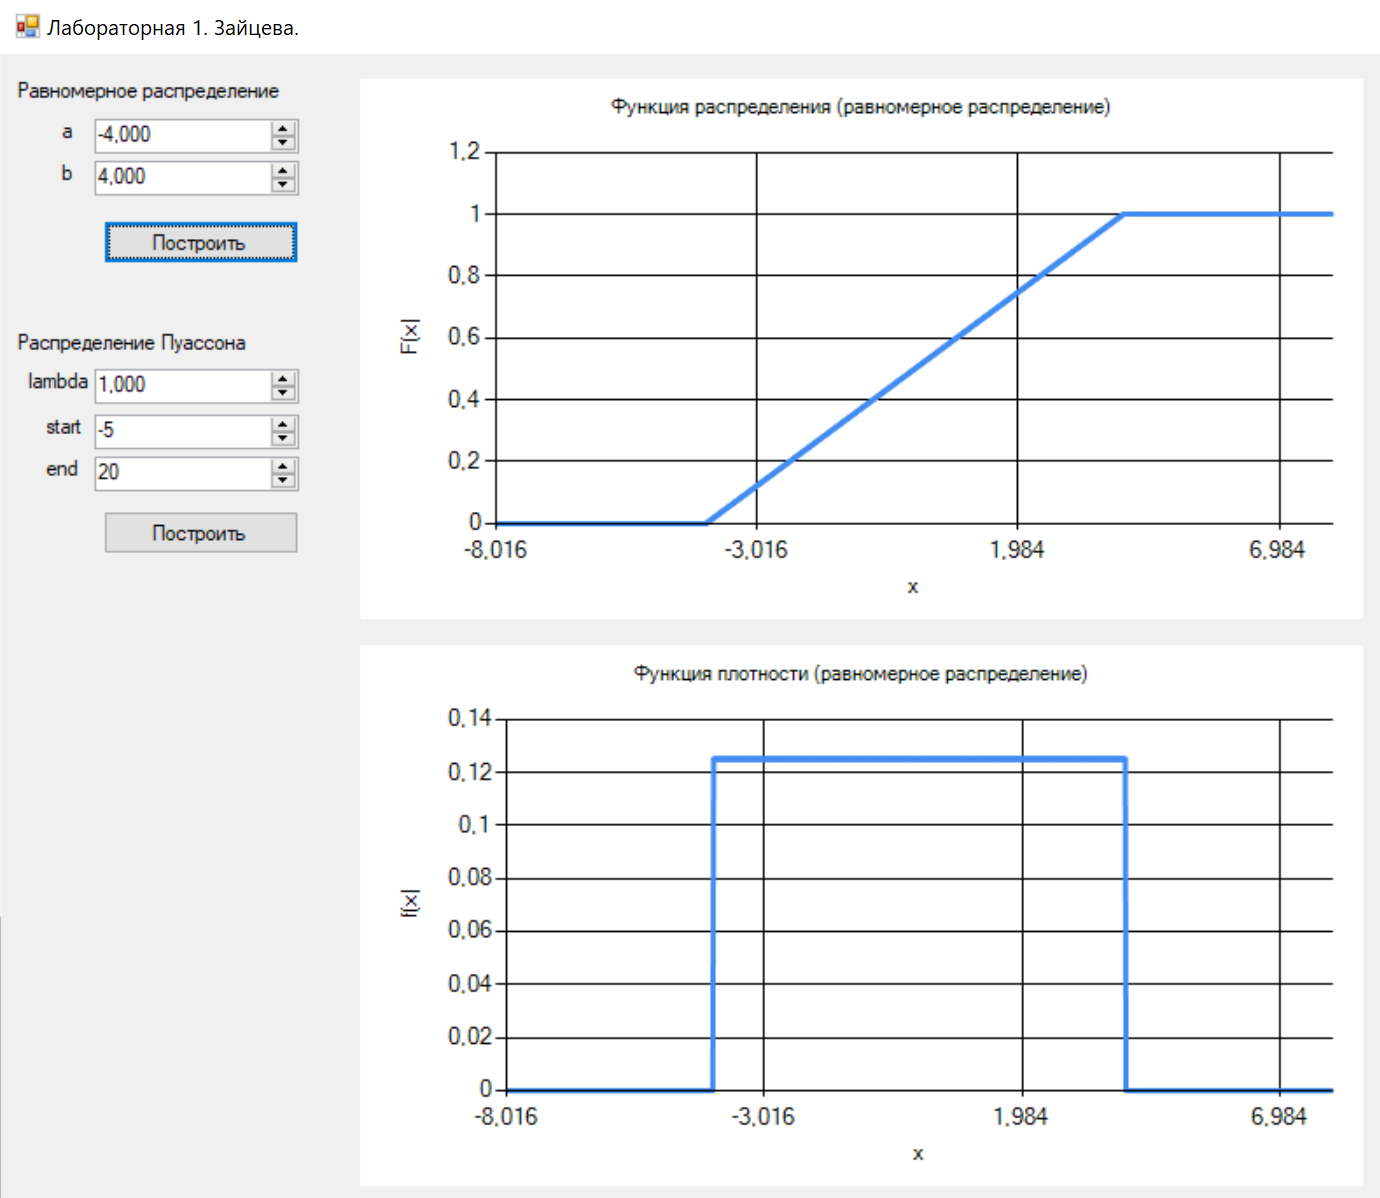
\includegraphics[scale=0.7]{pictures/u1.png}
	\end{center}
	\captionsetup{justification=centering}
	\caption{Графики функций плотности $f(x)$ и распределения $F(x)$ для случайной величины $X \sim R(-4, 4)$.}
	\label{fig:u1}
\end{figure}

\clearpage
\begin{figure}[h!]
	\begin{center}
		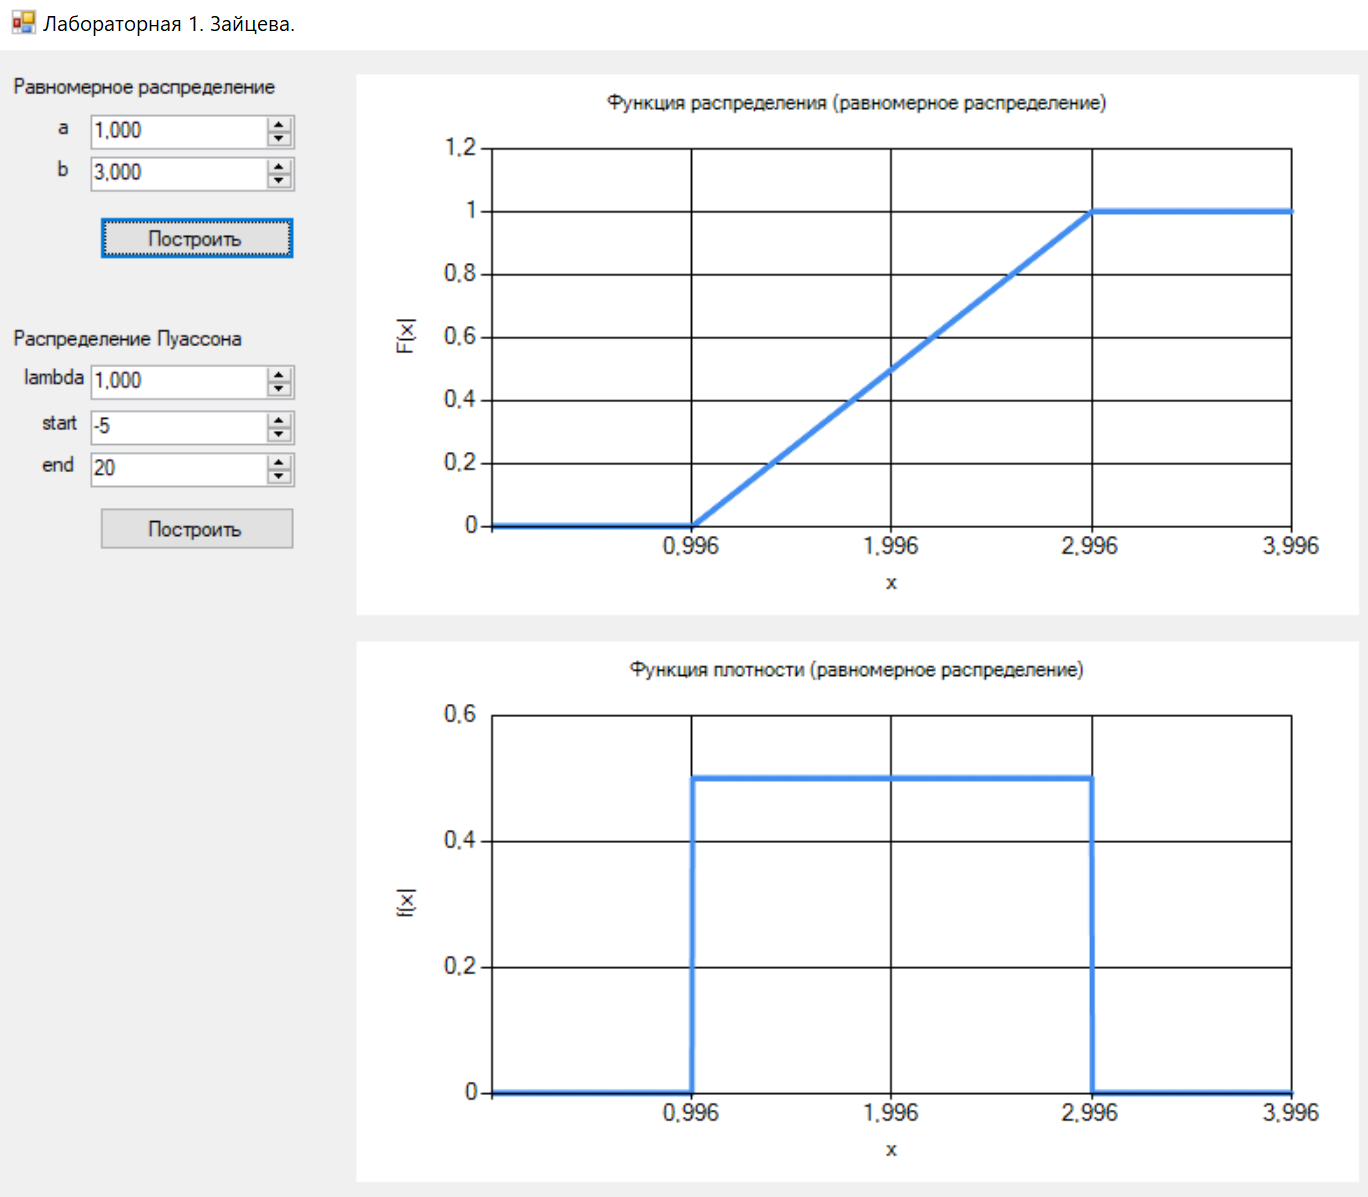
\includegraphics[scale=0.7]{pictures/u2.png}
	\end{center}
	\captionsetup{justification=centering}
	\caption{Графики функций плотности $f(x)$ и распределения $F(x)$ для случайной величины $X \sim R(1, 3)$.}
	\label{fig:u2}
\end{figure}



\subsection{Распределение Пуассона}

На рисунках \ref{fig:p1}, \ref{fig:p2} и \ref{fig:p3} приведены результаты построения графиков функции вероятности $P(x)$ и распределения $F(x)$ на отрезке $x \in [-3, 20]$ для случайных величин $X \sim \Pi(1)$, $X \sim \Pi(3)$ и $X \sim \Pi(10)$, соответственно.

\clearpage
\begin{figure}[h!]
	\begin{center}
		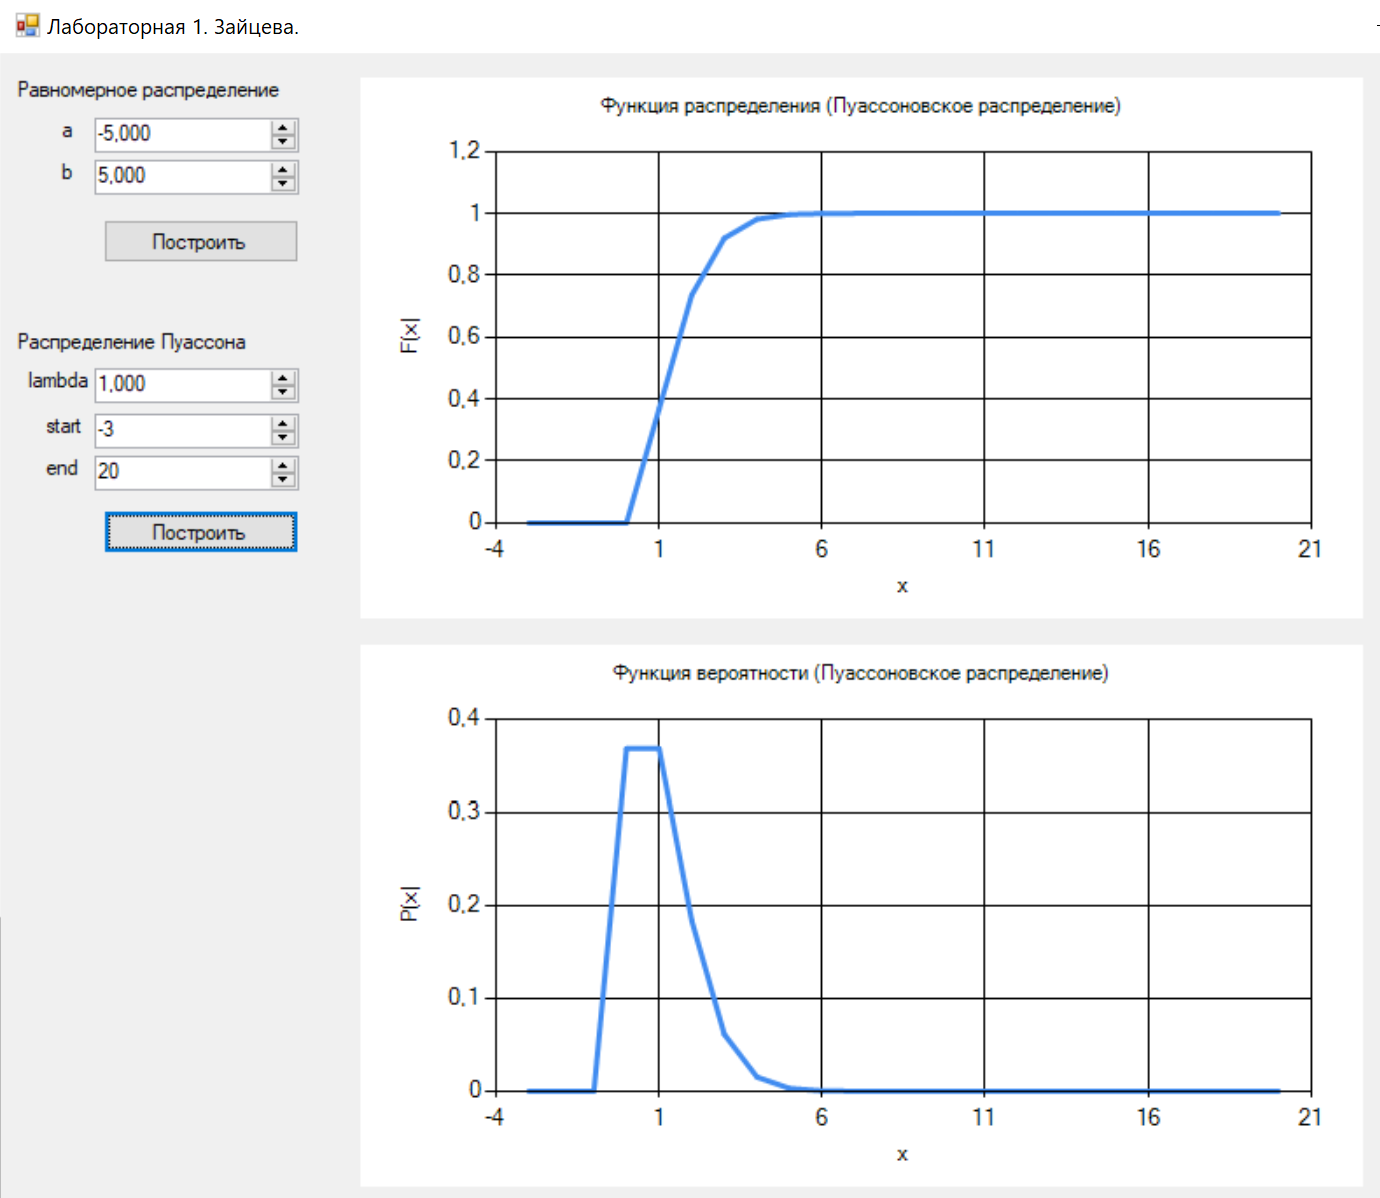
\includegraphics[scale=0.7]{pictures/p1.png}
	\end{center}
	\captionsetup{justification=centering}
	\caption{Графики функций вероятности $P(x)$ и распределения $F(x)$ для случайной величины $X \sim \Pi(1)$.}
	\label{fig:p1}
\end{figure}

\clearpage
\begin{figure}[h!]
	\begin{center}
		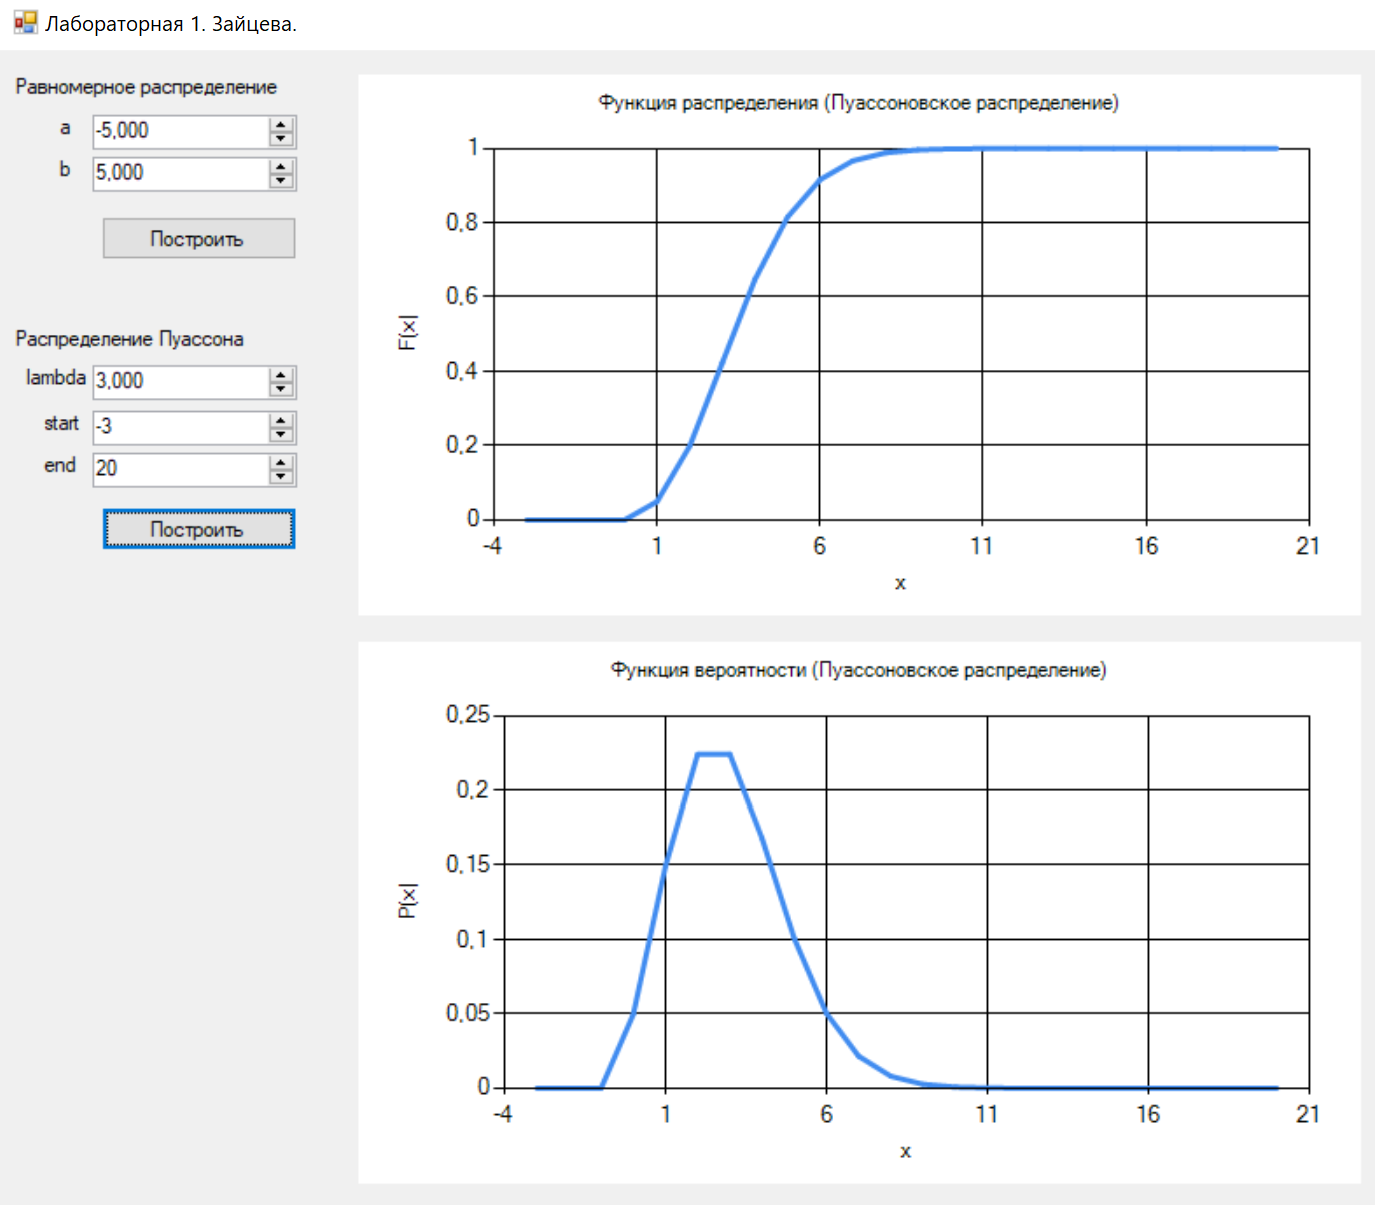
\includegraphics[scale=0.7]{pictures/p2.png}
	\end{center}
	\captionsetup{justification=centering}
	\caption{Графики функций вероятности $P(x)$ и распределения $F(x)$ для случайной величины $X \sim \Pi(3)$.}
	\label{fig:p2}
\end{figure}

\clearpage
\begin{figure}[h!]
	\begin{center}
		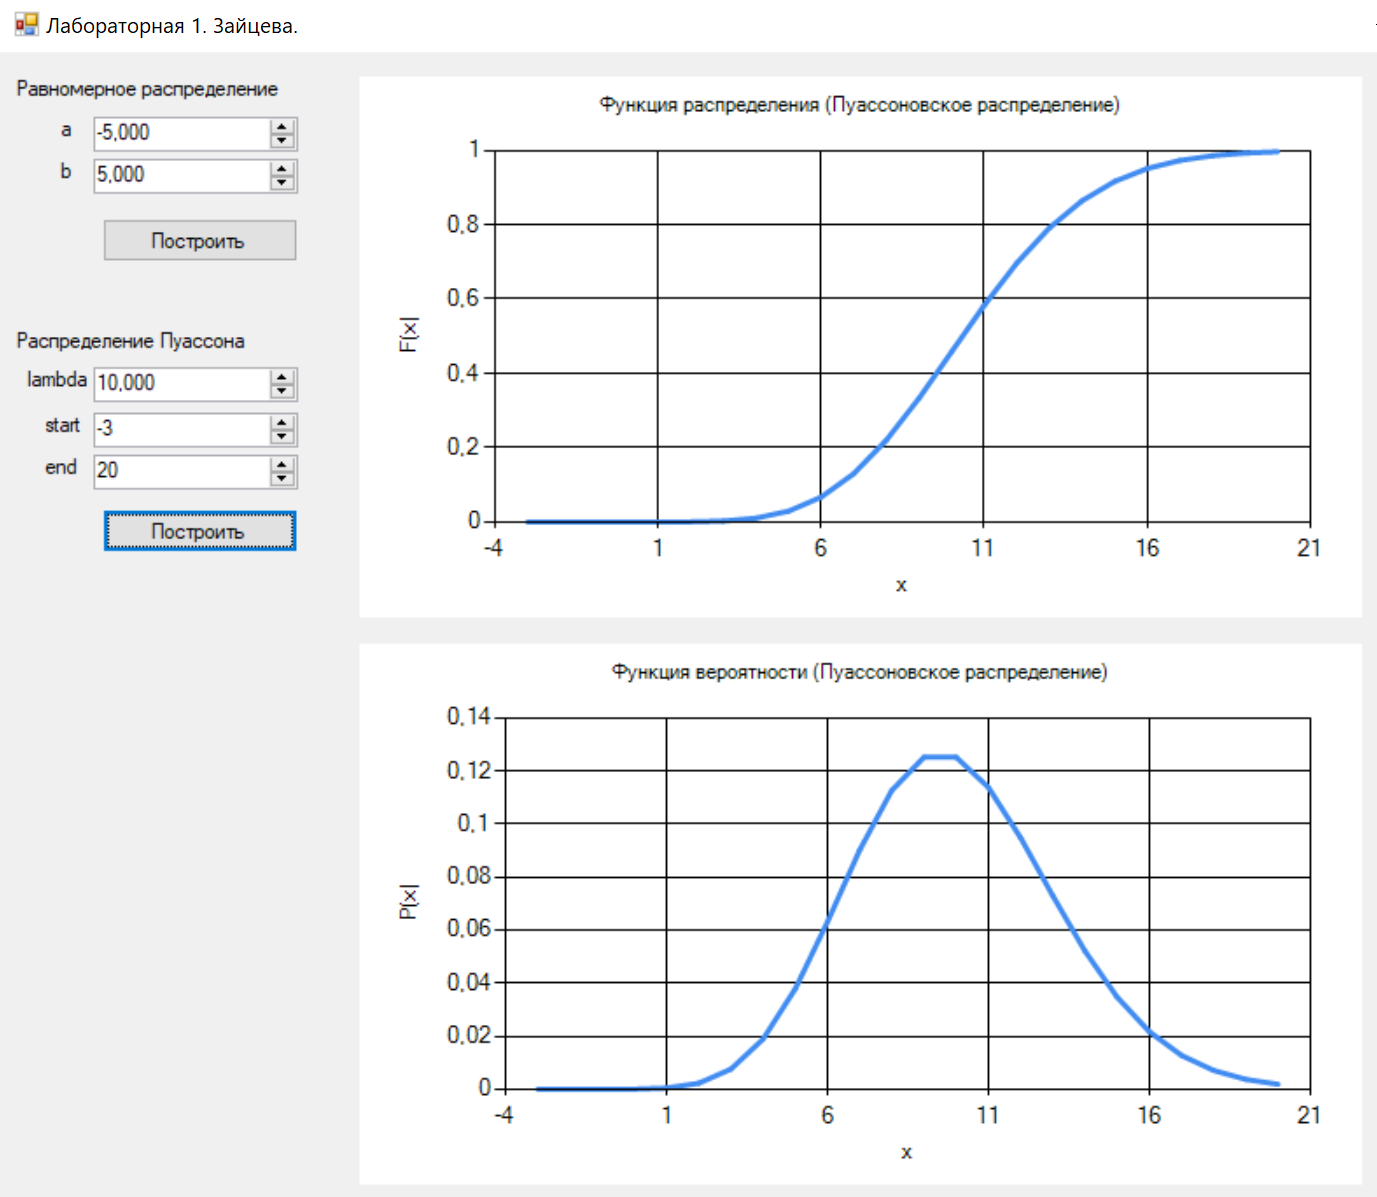
\includegraphics[scale=0.7]{pictures/p3.png}
	\end{center}
	\captionsetup{justification=centering}
	\caption{Графики функций вероятности $P(x)$ и распределения $F(x)$ для случайной величины $X \sim \Pi(10)$.}
	\label{fig:p3}
\end{figure}


\section{Код программы}

В листинге \ref{lst:list1} приведены классы и их методы, используемые для построения графиков функций (использованный язык программирования -- C\#).

\begin{lstlisting}[caption = {Реализация построения графиков функций}, label=lst:list1]
public class EqualDistribution
{
	private double a;
	private double b;
	private double p;
	
	public EqualDistribution(double a, double b)
	{
		this.a = a;
		this.b = b;
		this.p = 1 / (b - a);
	}
	
	private  double f(double x)
	{
		if ((x < a) || (x > b))
			return 0;
		else
			return p;
	}
	
	private double F(double x)
	{
		if (x < a)
			return 0;
		else if (x < b)
			return (x - a) * p;
		else
			return 1;
	}

	public void buildPlots(Chart chartDistr, Chart chartDens, double GraphStep = 1000)
	{
		var range = (b - a) * 2;
		var begin = (a + b - range) / 2;
		var end = (a + b + range) / 2;
		var step = range / GraphStep;
		
		for (double x = begin; x <= end; x += step)
		{
			chartDistr.Series[0].Points.AddXY(x, F(x));
			chartDens.Series[0].Points.AddXY(x, f(x));
		}
	}
}

public class PuassonDistribution
{
	private double lambda;
	private double exp_lambda;
	private int begin;
	private int end;
	
	public PuassonDistribution(double lambda, int begin, int end)
	{
		this.lambda = lambda;
		this.begin = begin;
		this.end = end;
		this.exp_lambda = Math.Exp(-this.lambda);
	}
	
	public double P(int x)
	{
		if (x < 0)
			return 0;
		else
			return exp_lambda * Math.Pow(lambda, x) / factorial(x);
	}
	
	public double F(int x)
	{
		if (x < 0)
			return 0;
		
		double sum = 0;
		for (int k = 0; k < x; k++)
			sum += P(k);
		
		return sum;
	}
	private long factorial(int n)
	{
		if (n < 2) return 1;
		
		return n * factorial(n - 1);
	}
	
	public void buildPlots(Chart chartDistr, Chart chartDens, double GraphStep = 1000)
	{
		int step = 1;
		
		for (int x = begin; x <= end; x += step)
		{
			chartDistr.Series[0].Points.AddXY(x, F(x));
			chartDens.Series[0].Points.AddXY(x, P(x));
		}
	}
}
\end{lstlisting}

\end{document}